\documentclass[../main.tex]{subfiles}

\begin{document}
	 \section{Die marktwirtschaftliche Legalisierung}
	 
	 \subsection{Definition}
	 Die marktwirtschaftliche Legalisierung ist eine Art der Legalisierung, bei der der Markt so wenig wie möglich eingeschränkt wird, so dass die Allokation der Ressourcen über den Marktpreis koordiniert wird.
	 Ein marktwirtschaftliches System ohne staatliche Regulierungen reguliert sich selbst und stellt sich beim ökonomischen Marktgleichgewicht ein.
	 
	 
	 
	 \subsection{Ein mögliches Schweizer Modell}
	 Die in der Arbeit angesprochene Legalisierung soll den Anspruch der Verdrängung des Schwarzmarktes so weit wie möglich erfüllen.
	 Das Nebenziel, gefährdete Gesellschaftsgruppen zu schützen, wird durch eine Legalisierung noch mehr gestärkt, da der Jugendschutz erst auf den legalen Markt einwirken kann.
	 Das potentielle Schweizer Konzept ist so aufgebaut, dass sowohl Konsum und Besitz als auch Handel und Anbau unter bestimmten Bedingungen legal ist.
	 Niemand soll am Markteintritt gehindert werden, solange er sich an die Rahmenbedingungen hält.
	 So wird neben dem Jugendschutz auch der Konsumentenschutz garantiert.
	 Das nächste existierende Konzept stellt der Kanadische Ansatz dar, der im Anhang genauer erklärt wird.
	 Auf die starke Besteuerung wie in Kanada wird jedoch im Schweizer Konzept verzichtet.\\
	 
	 \noindent
	 Ausser den unten genannten Einschränkungen soll die Ressourcenallokation dem freien Markt überlassen werden. 	 
	 Massnahmen zur Minderung der Prävalenzen gehen über die Nachfrageseite und nicht wie bei der Repression über die Angebotsseite.
	 Die Auswirkungen des Eingreifens werden im Kapitel \texttt{Die marktwirtschaftliche Legalisierung > Ökonomie > Preis} genauer erklärt.
	 
	 
	 \subsection{Ökonomie}
	 
	 \paragraph{Preis}
	 Bei einer marktwirtschaftlichen Legalisierung würde der Marktpreis sofort fallen, da sich der Preis beim Marktgleichgewicht eingliedern würde. 
	 Der Marktpreis würde sich dem Einstandspreis anpassen und die Ressourcenallokation wäre über den Markt gesteuert.
	 Eine zusätzliche Besteuerung ist kontraproduktiv, da sich der Preis des Schwarzmarktes auch im Bereich des Marktpreises einpendeln wird.
	 Dies beobachtet man zurzeit in Kanada, da die Differenz zwischen dem Durchschnitt von legalem (\$10.30) und illegalem Cannabis (\$5.73) immer grösser wird und einige Konsumenten wieder auf den Schwarzmarkt ausweichen.%
	 \footnote{Vgl. \cite{cbc-01}.}\\
	 
	 \noindent
	 Da die Repression komplett beseitigt wurde, wird das Angebot nicht mehr künstlich beeinflusst.
	 Ohne einschränkende Massnahmen würde sich ein Marktgleichgewicht wie auf der linken Seite der Abbildung \ref{fig:equilibrium-legalization} einstellen.
	 Die Prävention bietet eine Möglichkeit, das Marktgleichgewicht zu verändern, ohne dass die Preise steigen würde.
	 Der Unterschied der Prävention im Gegensatz zur Repression liegt darin, dass die Nachfrageseite und nicht die Angebotsseite beeinflusst wird.
	 Die Nachfrage verschiebt sich nach links, so dass sowohl die Menge als auch der Preis sinken würde.
	 Die Entwicklung sieht man auch auf der rechten Seite der Abbildung \ref{fig:equilibrium-legalization}.
	 
	 \begin{figure}[H]
	 \centering
	 \begin{minipage}{0.48\linewidth}
	 	\centering
		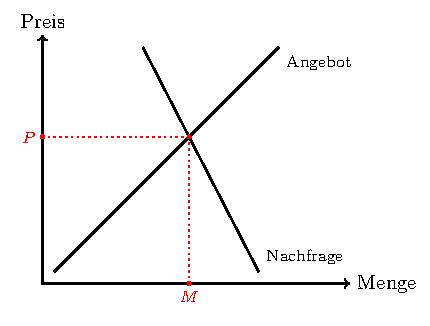
\includegraphics[width=\textwidth]{../figures/priceelasticity-equilibrium}
	 \end{minipage} 
	 \hfill
	 \begin{minipage}{0.48\linewidth}
	 	\centering
		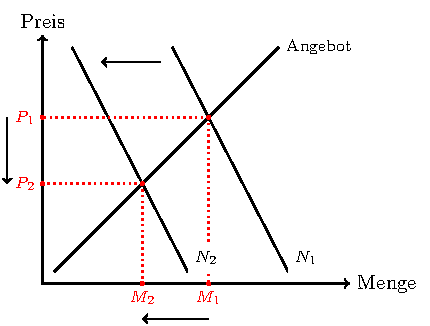
\includegraphics[width=\textwidth]{../figures/priceelasticity-prevention}
	 \end{minipage}
	 \captionsetup{font=small}
	 \caption[Preis-Mengen-Diagramm der Legalisierung]{Preis-Mengen-Diagramm der Legalisierung\protect\footnotemark}\label{fig:equilibrium-legalization}
	 \end{figure}	 
	 \footnotetext{Eigene Abbildung. Vgl. \cite[133-134]{mankiv-2018}.}
	 
	 \noindent
	 Im theoretischen Modell der marktwirtschaftlichen Legalisierung würde der Marktpreis um ein Vielfaches fallen.
	 Die Produktionskosten eines Cannabis Unternehmens können je nach Qualität und Grösse des Unternehmens stark schwanken.
	 Der Produktionspreis von Cannabis von kanadischen Unternehmen befindet sich zwischen \$1-3 pro Gramm und im Durchschnitt etwa \$2 pro Gramm.%
	 \footnote{Vgl. \cite{seekingalpha-01}.}
	 In Schweizer Unternehmen wird man nach einer Legalisierung ähnliche Produktionspreise antreffen. 
	 Auch wenn einige Kosten in der Schweiz höher
	 Einige Kosten werden in der Schweiz höher sein, v. a. Stromkosten und Löhne, während andere Kosten in der Schweiz tiefer sind, da im Konzept der Arbeit keine spezifische Cannabisbesteuerung vorgesehen ist.
	 Aus diesem Grund wird in den folgenden Berechnungen der kanadische Durchschnittspreis der Produktion von \$2 auch als Schweizer Produktionspreis verwendet.\\
	 \textit{($\approx$ CHF 1.80 bei einem Wechselkurs von \$1 $\approx$ CHF 0.90, Stand: 07.11.20)}
	 

	 \pagebreak	 
	 
	 \subsection{Rechtslage \& Einschränkungen}
	 
	 \subsubsection{Cannabisgesetz}
	 Die Legalisierung kann nicht ohne Einschränkungen erfolgen und deswegen muss man ein neues Gesetz in Betracht ziehen.
	 Als Beispiel dienen Gesetze über den Umgang mit Tabak und Alkohol.
	 Der gesetzliche Umgang mit Alkohol und mit Tabak, zwei legalen psychoaktiven Substanzen wird in eigenen Gesetzen geregelt. 
	 Aus diesem Grund müsste man für Cannabis ein neues Gesetz mit Verordnungen erlassen, das die Herstellung, Einfuhr und Ausfuhr, Verkauf und Besteuerung regeln würde.	 
	 Im Cannabisgesetz und in bereits bestehenden Gesetzen werden die in den folgenden Untersektionen genannten Einschränkungen weiter konkretisiert.
	 
	 \subsubsection{Besteuerung}
	 Das Ausmass der gesamten Besteuerung wird im Kapitel \texttt{Legalisierung > Besteuerung} ermittelt.
	 Das Ziel der marktwirtschaftlichen Legalisierung ist es, die Allokation der Güter möglichst dem Markt zu überlassen.
	 Die Rechtsgrundlage schafft nur die Möglichkeit zu einem späteren Zeitpunkt eine Besteuerung einzuführen. 
	 Sie ist jedoch kein Muss für den marktwirtschaftlichen Ansatz.\\
	 
	 \noindent
	 Eine Cannabissteuer muss schon auf der höchsten Stufe der Normenhierarchie geregelt werden. 
	 Die Rechtsgrundlage der Besteuerung wird der von Alkohol und Tabak gleichen, da es sich bei allen drei Produkten um psychoaktive Substanzen handelt.
	 Die besondere Verbrauchssteuer nach \texttt{Art. 131 Abs. 1 BV} muss so erweitert werden, dass der Bund diese auch auf Cannabis und dessen Produkte erheben kann.
	 Die Einnahmen der Verbrauchssteuern sollen in Prävention und Behandlung von Suchtproblemen aber auch in die vorhandenen Ausgleichskassen fliessen.
	 Mit der Erweiterung von \texttt{Art. 131 Abs. 3 BV} für Prävention und Therapie und \texttt{Art. 112 Abs. 5 BV} für die AHV und IV mit Cannabis, ist die Grundlage für eine Besteuerung geebnet.
	 	 
	 \noindent
	 Nähere Bestimmungen über die Besteuerung würden im neuen Cannabisgesetz festgelegt werden.
	 Es existieren viele Faktoren, die sich für eine Besteuerungsgrundlage eignen würden, jedoch bewies sich die Besteuerung nach absolutem Inhalt bereits zahlreich.
	 Tabak- und Alkoholprodukte werden nach gleichem Prinzip besteuert und tragen einen wesentlichen Teil der Deckung der Schäden bei.
	 Auch Ausgleichskassen wie die AHV oder IV werden durch die Steuerlast der Produkte teilfinanziert.
	 Eine Besteuerung nach absolutem THC Gehalt ist der gewichtsbasierten Besteuerung zu bevorzugen, da sich dann keine Anreize für die Hersteller ergeben, den THC Gehalt künstlich hochzuzüchten.
	 Eine höhere Besteuerung auf potenteres Cannabis sollte chronische Konsumenten abhalten, potenteres Cannabis zu konsumieren, das einen höheren Schaden verursacht.  
	 
	 \paragraph{Mehrwertsteuer}
	 Die Mehrwertsteuer ist eine universelle Steuer und wird auf den Bruttoverkaufspreis erhoben.
	 Sie ist im Bundesgesetz über die Mehrwertsteuer (MWSTG) geregelt.
	 Nach \texttt{Art. 25 Abs. 1 MWSTG} beträgt der Normalsatz 7.7\% und der reduzierte Satz 2.5\%.
	 Für den grössten Teil des Marktvolumens gilt der Normalsteuersatz, da wir von THC-haltigem Cannabis ausgehen, das rein zum Freizeitkonsum dient und keinerlei medizinische Zwecke hat. 
	 Der Anteil der medizinischen Anwendungen von THC ist noch so klein, dass man ihn vernachlässigen kann.\\
	 
	 \noindent
	 Der Einstandspreis eines Gramms Cannabis stellt den Nettopreis des Produktes dar.
	 Den Bruttopreis kann man mit einer einfachen Prozentrechnung (siehe Formel \ref{equ:brutto}) ausrechnen. 
	 Die Mehrwertsteuer pro Gramm Cannabis ist die Differenz von Brutto- und Nettopreis.
	 Das gesamte Steuereinkommen durch die Mehrwertsteuer lässt sich mit der Formel \ref{equ:mwst} berechnen.\\
	 
	 \noindent
	 \begin{align}
	 	 \text{Bruttopreis} &= \text{Nettopreis} \cdot \left( 1 + \frac{\text{Mehrwertsteuersatz}}{100} \right)\label{equ:brutto} \\[7pt]
	 	\text{Gesamte Mehrwertsteuer} &= \text{Menge} \cdot \underbrace{\left(\text{Bruttopreis} - \text{Nettopreis} \right)}_{\text{Mehrwertsteuer pro Gramm}} \label{equ:mwst} 
	 \end{align}
	 
	 \noindent\\
	 Die erste Berechnung der Mehrwertsteuer erfolgt unter der Annahme, dass es sich um eine marktwirtschaftliche Legalisierung ohne Verbrauchssteuer handelt.
	 Als Nettopreis wird der Einstandspreis eines verkäuflichen Gramms Cannabis genommen.
	 Der durchschnittliche Einstandspreis des verkäuflichen Produktes wurde im Kapitel 2.3 ermittelt.
	 Das Endergebnis der Berechnung ist ein Intervall, da man das Marktvolumen eines Schwarzmarktes nicht genau bestimmen kann. 
	 Die Steuereinnahmen der Mehrwertsteuer beim marktwirtschaftlichen Ansatz würden sich auf CHF 5.25 Mio. bis CHF 7.685 Mio. belaufen.
	 \textit{(Siehe Tabelle \ref{table:mwst-legal})}
	 
	 \noindent
	 \captionsetup{font=small}
	 \captionof{table}{Berechnung der Mehrwertsteuer ohne Verbrauchssteuer}
	 \label{table:mwst-legal}
	 \begin{tabularx}{\textwidth}{X p{3.5cm} p{2.5cm} p{3.5cm}}
     	\toprule
     	\phantom{x} & Minimum & & Maximum \\
        \midrule
        Menge & 37.5 Tonnen & & 54.7 Tonnen\\
        \midrule
        Nettopreis & & CHF 1.80 & \\
        \midrule
        Bruttopreis & & CHF 1.94 & \\
        \midrule
        Mehrwertsteuer pro Gramm & & CHF 0.14 & \\
        \midrule
        Gesamte Mehrwertsteuer & CHF 5.25 Mio. & & CHF 7.685 Mio\\
        \bottomrule
     \end{tabularx}\pagebreak
     
     \noindent
     Die Mehrwertsteuer unter dem zurzeit vorzufindenden Preisniveau würde sich auf CHF 26.625 Mio. bis CHF 38.837 Mio. belaufen.
     Dieser Wert der Mehrwertsteuer ist jedoch rein theoretisch und könnte nur mit einer Cannabissteuer erreicht werden.
	 \textit{(Siehe Tabelle \ref{table:mwst-illegal})}
     
     \noindent
	 \captionsetup{font=small}
	 \captionof{table}{Berechnung der hypothetischen Mehrwertsteuer der Prohibition}
	 \label{table:mwst-illegal}
	 \begin{tabularx}{\textwidth}{X p{3.5cm} p{2.5cm} p{3.5cm}}
     	\toprule
     	\phantom{x} & Minimum & & Maximum \\
        \midrule
        Menge & 37.5 Tonnen & & 54.7 Tonnen \\
        \midrule
        Nettopreis & & CHF 10.21 & \\
        \midrule
        Bruttopreis & & CHF 11.00 & \\
        \midrule
        Mehrwertsteuer pro Gramm & & CHF 0.79 & \\
        \midrule
        Gesamte Mehrwertsteuer & CHF 29.625 Mio. & & CHF 43.213 Mio.\\
        \bottomrule
     \end{tabularx}\\
	 
	 
	 
	 
	 \paragraph{Cannabissteuer}
	 Die Verbrauchssteuer auf Cannabis steht im Gegensatz mit dem in der Arbeit besprochenen marktwirtschaftlichen Ansatz der Legalisierung.
	 Dennoch ist sie ein gutes Mittel, um die Nachfrage steuern zu können, falls man mit präventiven Massnahmen nicht zum gewünschten Erfolg kommen würde.
	 Dies impliziert, dass die Verbrauchssteuer nicht für eine Erhöhung des Staatsbudget missbraucht werden sollte.	 
	 
	 \noindent
	 \captionsetup{font=small}
	 \captionof{table}{Berechnung der Cannabissteuer}
	 \label{table:cannabissteuer}
	 \begin{tabularx}{\textwidth}{X p{3.5cm} p{2.5cm} p{3.5cm}}
     	\toprule
     	\phantom{x} & Minimum & & Maximum \\
        \midrule
        Menge & 37.5 Tonnen & & 54.7 Tonnen \\
        \midrule
        Einstandspreis & & CHF 1.80 & \\
        \midrule
        Bruttopreis & & CHF 5.16 & \\
        \midrule
        Nettopreis & & CHF 4.79 & \\
        \midrule
        Mehrwertsteuer pro Gramm & & CHF 0.37 & \\
        \midrule
        Cannabissteuer pro Gramm & & CHF 2.99 & \\
        \midrule
        Gesamte Mehrwertsteuer & CHF 13.875 Mio. & & CHF 20.239 Mio.\\
        \midrule
        Gesamte Cannabissteuer & CHF 112.125 Mio. & & CHF 163.553 Mio.\\
        \midrule
        Gesamte Steuereinnahmen & CHF 126.0 Mio. & & CHF 183.792 Mio.\\
        \bottomrule
     \end{tabularx}\\ \\ \\
     
     \noindent	 
	 Am Beispiel Kanada konnte man sehen, dass der Preis von illegalem Cannabis auf \$5.73 sank und nur noch leicht in Zukunft sinken wird.
	 Um dem Schwarzmarkt entgegenzuwirken, wird der Verkaufspreis maximal bis zum Preis des Schwarzmarktes angehoben, so dass Kunden keine Anreize mehr haben, illegales Cannabis zu erwerben.
	 Aus diesem Grund wird der Bruttopreis in der Berechnung bei CHF 5.16 angesetzt.\\
	 \textit{($\approx$ CHF 5.16 bei einem Wechselkurs von \$1 $\approx$ CHF 0.90, Stand: 07.11.20)} \\
	 
	 \noindent
	 Die Cannabissteuer würde sich im Intervall zwischen CHF 112.125 Mio. und CHF 163.553 Mio. befinden.	 
	 Die gesamten Steuereinnahmen bei einer Preismanipulation auf das Preisniveau von illegalem Cannabis würden sich auf CHF 126.0 Mio. bis CHF 183.792 Mio. belaufen.\\
	 \textit{(Siehe Tabelle \ref{table:cannabissteuer})}
	 
	 \subsubsection{Jugendschutz}
	 In erster Linie dient der Jugendschutz dem Wohle der Kinder und Jugendliche, dass sie von den Risiken des Betäubungsmittelkonsums geschützt werden und ihre psychische und physische Entwicklung nicht beeinträchtigt wird. 
	 Eine bereits existierende Einschränkung im Jugendschutz stellt das Abgabealter von Alkohol an Jugendliche dar, das sich bei 18 Jahren befindet (\texttt{Art. 41 Abs. 1 lit. i AlkG}). 
	 Bei Cannabis würde man auch ein Schutzalter zwischen 18 - 20 Jahren anstreben. 
	 Dies ist sinnvoll, da die Gehirnentwicklung des Menschen sich ab dem 18. Lebensjahr verlangsamt und bei ungefähr 25 Jahren weitgehend abgeschlossen ist.%
	 \footnote{Vgl. \cite{arain-2013}.}
	 Zwar ist die Gehirnentwicklung bei einem 18-jährigen Erwachsenen noch nicht vollständig abgeschlossen, jedoch kann man annehmen, dass eine Person ab diesem Alter mehr Eigenverantwortung übernehmen kann.
	 Es wäre kontraproduktiv, einem Teil der grössten Gruppe an Konsumenten den Zugang zum legalen Markt zu verweigern, da diese sonst auf den Schwarzmarkt ausweichen.\\
	 
	 \noindent
	 Der Kern des Jugendschutzes besteht zwar primär aus einem Abgabeverbot an Jugendliche, jedoch müssen auch alle anderen Massnahmen der Vier-Säulen-Politik umgesetzt werden. 
	 Als direkte Auswirkung folgt, dass bereits konsumierende Jugendliche Hilfe bei der Bewältigung ihrer Sucht zur Verfügung gestellt bekommen. 
	 Neben der Suchthilfe für chronische Konsumenten ist auch die Früherkennung und Intervention von grosser Bedeutung. 
	 Durch eine Legalisierung wird der Konsum nicht mehr stark stigmatisiert, sodass Bezugspersonen die Situationen frühzeitig erkennen und handeln können. 
	 Die Prävention erhalten alle Jugendliche, sodass Kinder und Jugendliche wichtige Kompetenzen erlernen, sich gegen den Konsum von Betäubungsmitteln zu stellen.  
	 
	 \subsubsection{Werbeeinschränkungen}
	 Die Viersäulenpolitik der Schweizer Drogenpolitik gibt das Ziel vor, den Konsum von psychoaktiven Substanzen so weit wie möglich zu mindern.
	 Ein gutes Marketing bewirkt das Gegenteil, es führt zu einer Erhöhung der Absatzzahlen.
	 Den Unternehmen sind ohne Einschränkungen unzählige Möglichkeiten geboten, ihr Produkt so positiv wie möglich darzustellen.	 
	 Vor allem Jugendliche und junge Erwachsene können durch Werbung stark beeinflusst werden.
	 Als Beispiel dient dabei Werbung für Tabakprodukte und für Alkohol.
	 Viele Unternehmen in diesen Bereichen sind zwar der Meinung, dass ihre Werbung nicht jüngere Menschen beeinflussen würde, jedoch wurde dies in mehreren Studien widerlegt.
	 Sowohl Werbung für Tabak\footnote{Vgl. \cite{lovato}.} als auch für Alkohol\footnote{Vgl. \cite{jernigan}.} kann das Konsumverhalten beeinflussen.
	 Manche Werbungen vermitteln ein positives Gefühl und zeigen eine gewisse Normalität auf. 
	 So wird den Menschen nur positive Effekte vermittelt, während negative Effekte nicht erwähnt werden.
	 Da es sich bei allen Produkten um psychoaktive Substanzen handelt, kann man diese Beobachtungen auf Cannabisprodukte ableiten.
	 Das Ziel der Einschränkungen ist nicht, Werbung komplett zu verbieten, sondern sie so zu regulieren, dass sie keine falschen Informationen vermittelt.\\
	 
	 \noindent	 
	 Einschränkungen über die Werbung von Cannabis würden im Cannabisgesetz geregelt werden und würden dem Vorbild des Alkoholgesetzes, namentlich \texttt{Art. 42b AlkG}, folgen.
	 Der Kerngedanke der Einschränkungen besteht daraus, dass Nichtkonsumierende kein falsches Bild von den Produkten bekommen und nicht zum Konsum verleitet werden.
	 Der Begriff von Werbung beschränkt sich nicht nur auf digitale Werbung im Fernsehen oder auf Plakaten, sondern auch auf Wettbewerbe, Sponsorings und weiteren Kundenbindungsmassnahmen.
	 
	 	 
	 \subsubsection{Strassenverkehrsgesetz}
	 Unter aktueller Rechtslage herrscht ein komplettes Verbot von Cannabis im Strassenverkehr. 
	 Dies ist unter anderem dem zuzuschreiben, dass der Inhaltsstoff THC akut negative Effekte auf die kognitiven Fähigkeiten haben kann.	 
	 In der Verkehrsregelnverordnung nach \texttt{Art. 2 Abs. 2 VRV} führt schon der geringste Anteil an THC zur Fahrunfähigkeit.
	 Im Gegensatz zu Alkohol gilt für Cannabis die Nulltoleranz im Strassenverkehr.
	 Als Nachweis gilt schon die extrem geringe Menge von 1.5 µg/L nach \texttt{Art. 34 VSKV-ASTRA}.
	 Der Wert bleibt jedoch noch stundenlang über diesem Grenzwert, ohne dass der Konsument eine Wirkung spürt.
	 Bei regelmässigen Konsumenten existiert das Problem, dass das sich THC im Fettgewebe anreichern kann, sodass der Wert auch noch Tage danach über dem Grenzwert wäre. \\
	 
	 \noindent	 
	 In einer Studie wurde ermittelt, dass von Fahrern mit einer Konzentration von 8.2 µg/L im Blut ein ähnliches Unfallrisiko ausgeht wie von Fahrern mit einer Alkoholkonzentration von 0.5 Promille.%
	 \footnote{Vgl. \cite{hartman-2015}.}
	 Man hat festgestellt, dass Fahrer, die Cannabis konsumiert haben, teilweise von der idealen Fahrbahn abwichen.
	 Fahrer mit THC Einfluss stellen aber im Gegensatz zu alkoholisierten Fahrern dennoch eine kleinere Gefahr dar, da sie keine erhöhte Bereitschaft zum Beschleunigen zeigen und die Fahrbahn nicht häufiger verlassen.
	 Die Gleichstellung der Blutkonzentration von THC und Alkohol bezieht sich somit nur auf das Halten der idealen Fahrbahn.\\
	 
	 
	 \noindent	 
	 \begin{figure}[H]
	 	\centering
		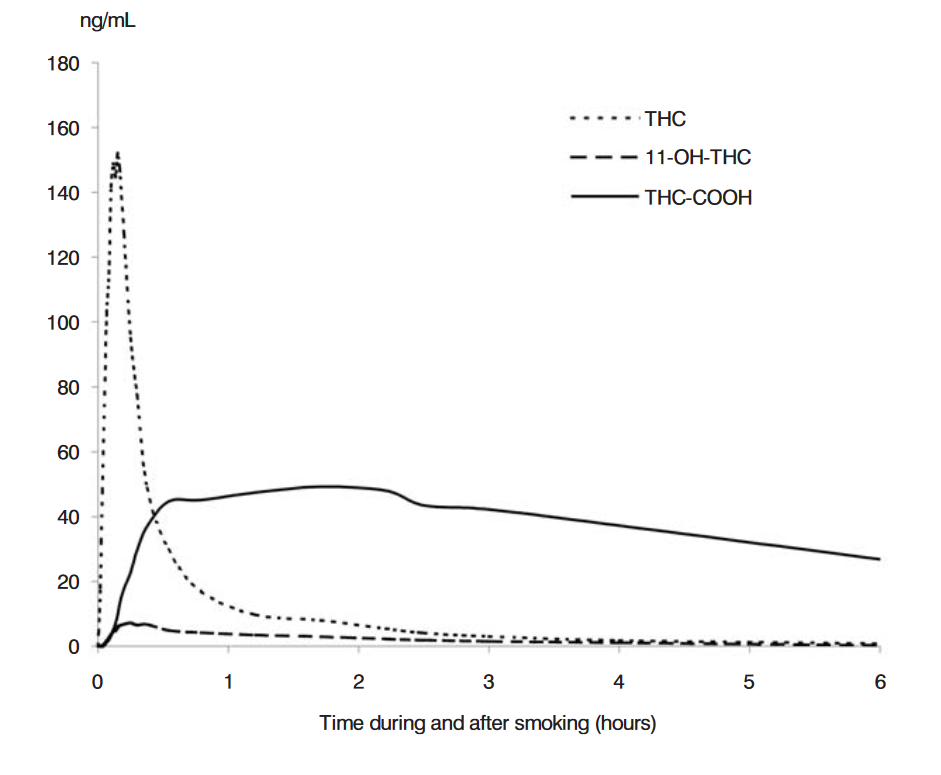
\includegraphics[height=9cm]{THCKonzentration}
		\captionsetup{font=small}
		\caption[Entwicklung der THC Konzentration im Blut]{Entwicklung der THC Konzentration im Blut\protect\footnotemark}		
	 \end{figure}
	 \footnotetext{\cite{giroud}}
	
	 \noindent
	 Mit einer Legalisierung sollte ein Grenzwert in Betracht gezogen werden.
	 Der Grenzwert sollte sich am bereits bestehenden Alkoholgrenzwert von 0.5 Promille orientieren. 
	 Vor allem sinnvoll wäre dieser Grenzwert für regelmässige Konsumenten, bei denen der Wert nur langsam sinkt.
	 Mit der neuen Regelung wären regelmässige Konsumenten bereits nach mehreren Stunden rechtlich wieder fahrfähig.	 
	 

\end{document}